%! Author = Stefan de Kraker
%! Date = 12-11-2021

% Preamble
\documentclass[11pt]{article}
\usepackage[english]{babel}
\renewcommand{\familydefault}{\sfdefault}
\NeedsTeXFormat{LaTeX2e}

\usepackage[paper=a4paper, top=1in, bottom=1.75in, left=1in, right=1.25in]{geometry}
\usepackage{graphicx}
\usepackage{float}
\usepackage{xcolor}
\usepackage{hyperref}
\usepackage{fancyhdr}
\usepackage{datetime}
\usepackage{booktabs}
\usepackage{adjustbox}
\usepackage{array}
\usepackage{csquotes}
\usepackage{pdfpages}
\usepackage[printonlyused,withpage]{acronym}
\usepackage[list=true,listformat=simple]{subcaption}
\usepackage{paralist}
\usepackage{vhistory}


% Setup Link in the docu
\hypersetup{
    filecolor=magenta,
    urlcolor=cyan,
    pdfpagemode=FullScreen,
    pageanchor=false
}
\usepackage[nameinlink]{cleveref}

% Header
\pagestyle{fancy}
\fancyhf{}
\setlength{\headheight}{33pt}
\lhead{Stefan de Kraker\\ HBO-ICT, Technische Informatica,\hspace{1mm} \today }
\rhead{\includegraphics[height=1cm]{C:/Work/latex-hva/alg_img/logo-hva.png}}
% Footer
% Center odd and even
\fancyfoot[C,CO]{\leftmark}
% Right odd and even
\fancyfoot[C]{page \thepage}
\renewcommand{\footrulewidth}{1.pt}

% Document
% Document
\begin{document}
    \begin{titlepage}
        \begin{center}
            \vspace*{0.3cm}

            \Huge
            \textbf{User manual}

            \vspace{0.5cm}
            \LARGE
            Crypt-o-meter\\

            \vspace{0.8cm}

%            \includegraphics[width=0.7\textwidth]{img/front}x

            \Large
            Hogeschool van Amsterdam\\
            Stefan de Kraker, 500823223\\
            \today

            \vspace{0.8cm}


        \end{center}
    \end{titlepage}
    \newpage
    \begin{versionhistory}
        \vhEntry{1.0}{12.11.21}{SDK}{First version}
        \vhEntry{1.1}{12.11.21}{SDK}{Added User inferface explanation}
    \end{versionhistory}
    \newpage
    \tableofcontents
    \newpage
    \section{Introduction}\label{sec:introduction}
    Thank you for getting the Crypt-o-meter, this little device will help u keep track of your crypto coins.
    In this user manual we will help you setup up your devices.

    \section{Setting up the Crypt-o-meter}\label{sec:setting-up-the-Crypt-o-meter}
    For setting up the device, you needs 3 things:
    \begin{itemize}
        \item 5V usb charger
        \item Usb A to B mini cable
        \item A active WiFi connection
    \end{itemize}
    If all of these things are all available then proceed the setup, else the setup cant be done.

    \paragraph{1} Plug in the usb A to B mini cable in to the charger and device.
    The B mini side fits the Crypt-o-meter, the other side should fit into any standard 5V charger that is made to charge your phone or table.
    \paragraph{2} Plug the usb charger in and wait for the Crypt-o-meter to show you the following screen.
    On this screen you will see that the Crypt-o-meter has made a wifi point named ``To the moon setup''~(\textcolor{blue}{\cref{fig:firt_setup}}).

    \begin{figure}[H]
        \centering
        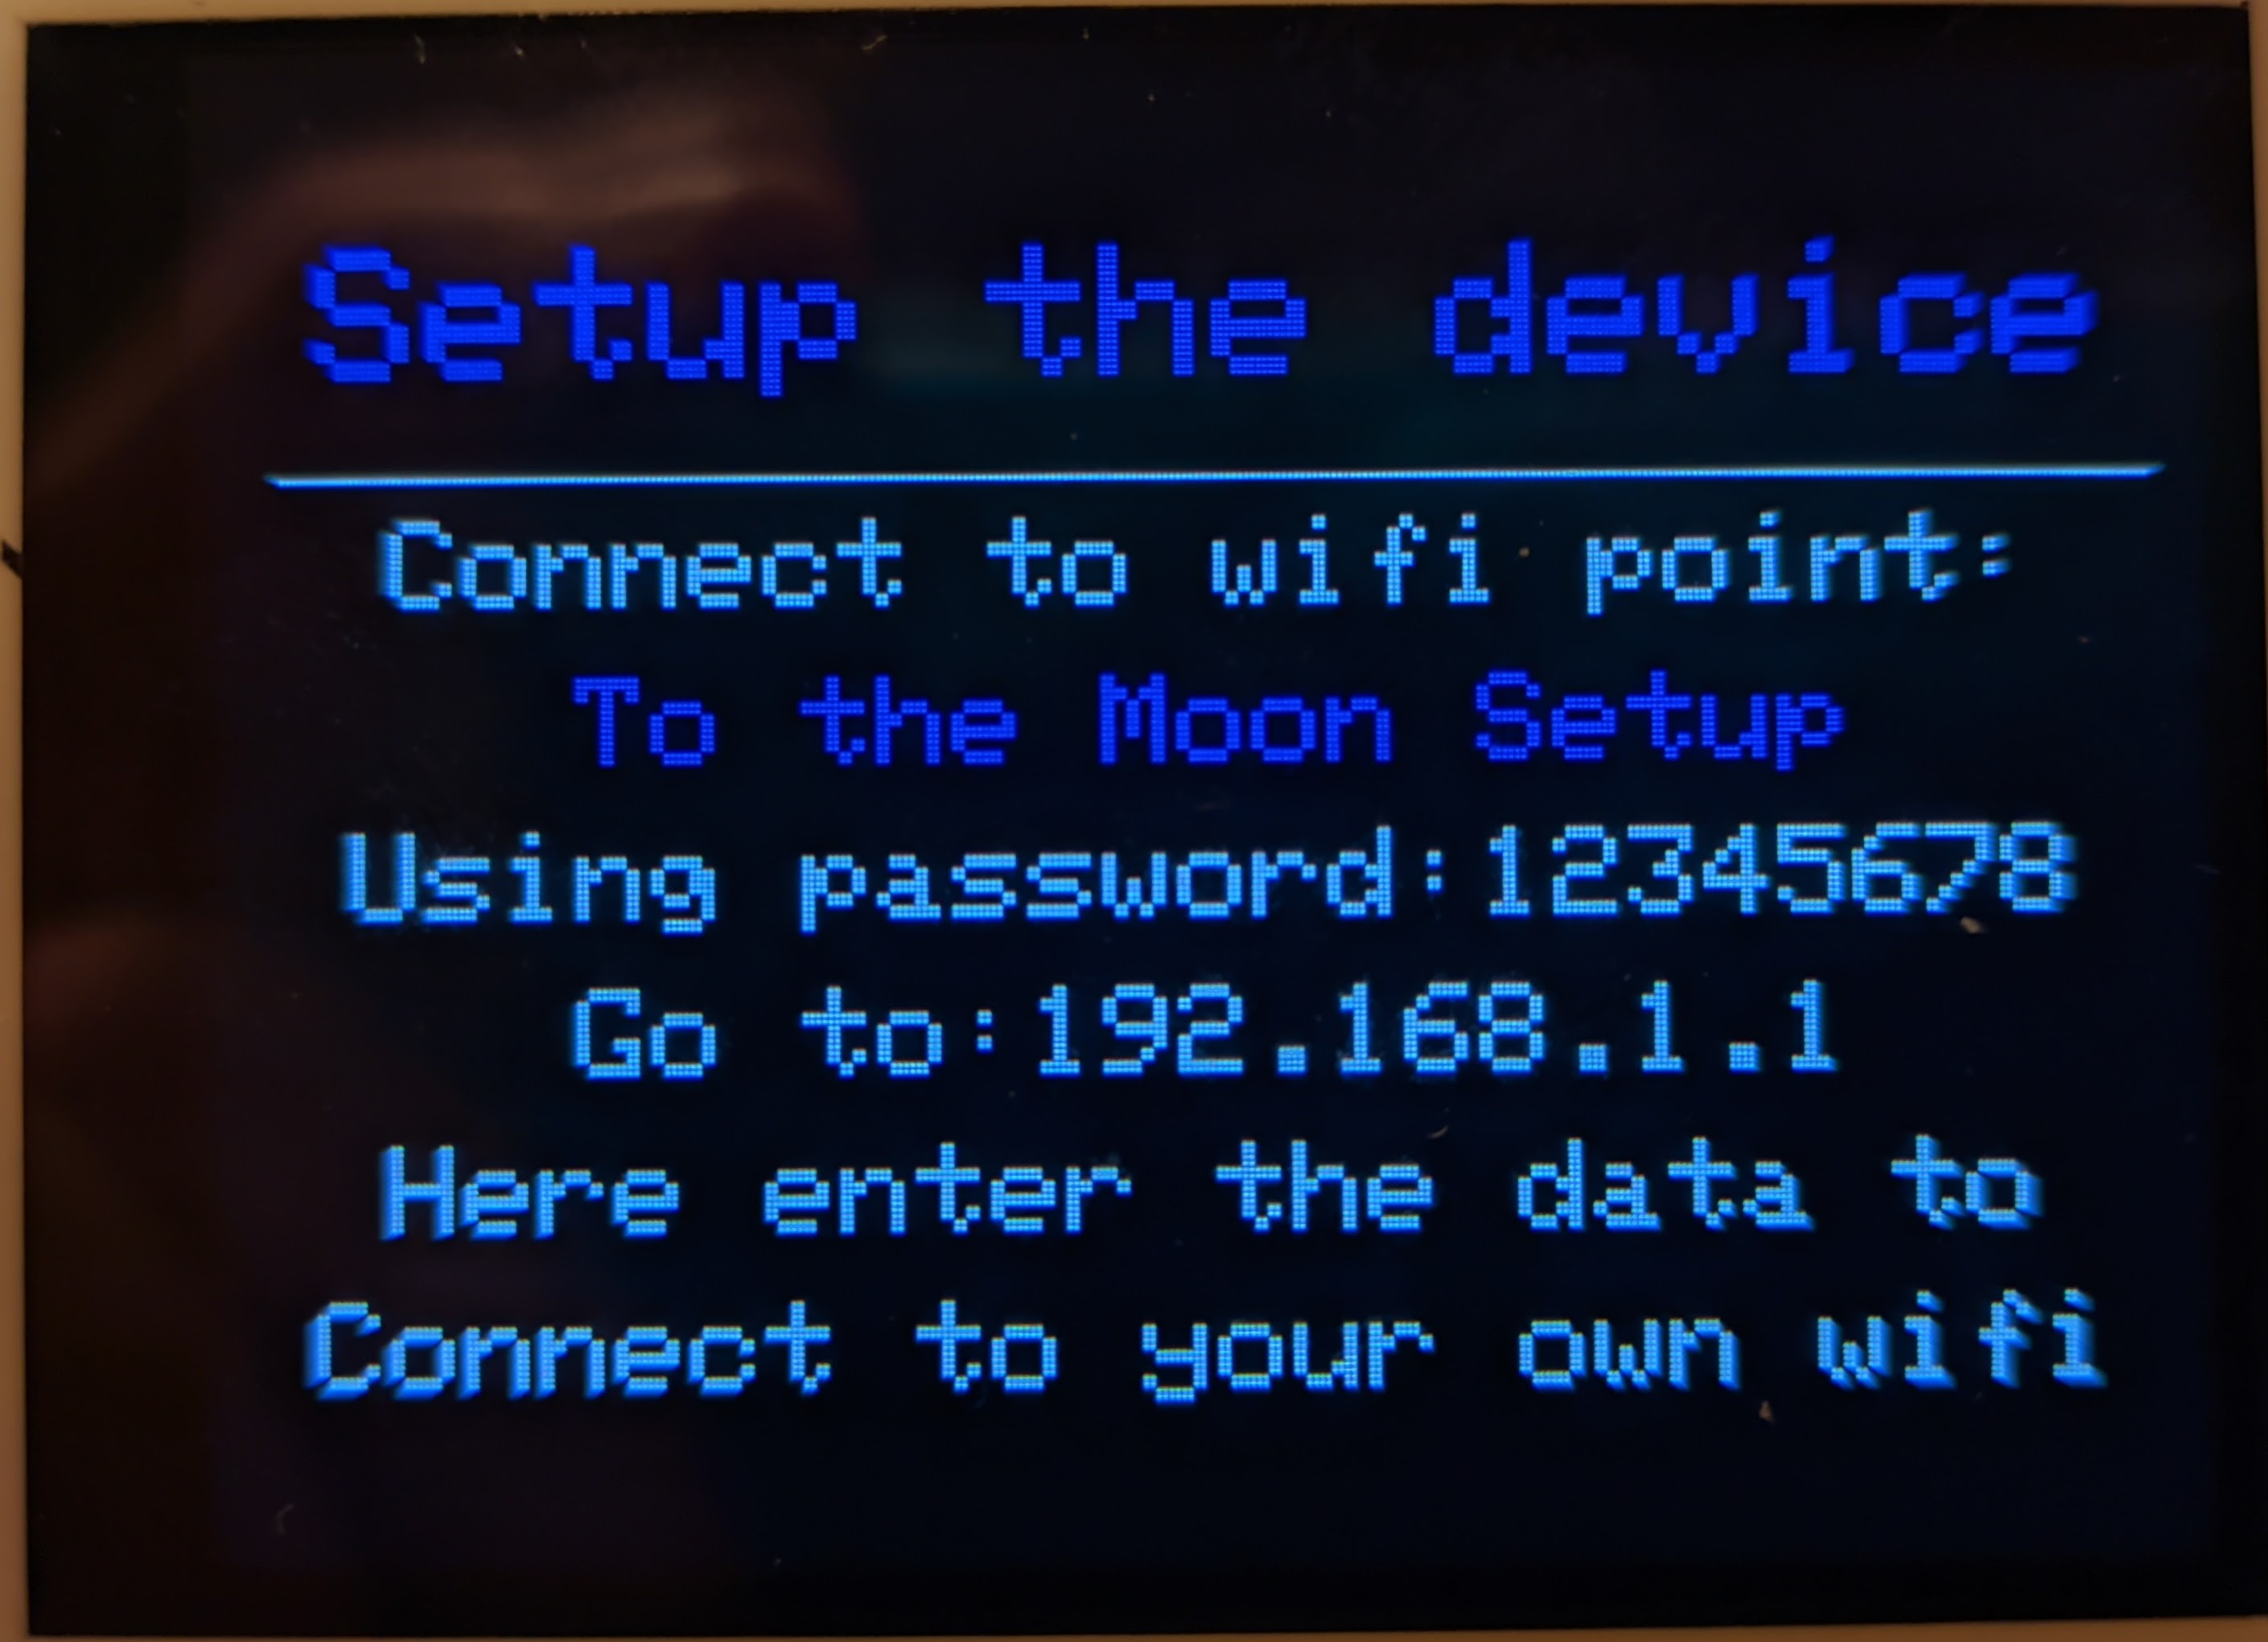
\includegraphics[width= 0.6\textwidth]{step_1}
        \caption{First setup screen of the Crypt-o-meter}
        \label{fig:firt_setup}
    \end{figure}
    
    \newpage

    \paragraph{3} Connect to this wifi acces point ~(\textcolor{blue}{\cref{fig:step_2}}) with your phone or laptop using the password given below, ``12345678'' in this case~(\textcolor{blue}{\cref{fig:step_3}}).
    \begin{figure}[H]
        \centering
        \begin{minipage}{0.45\textwidth}
            \centering
            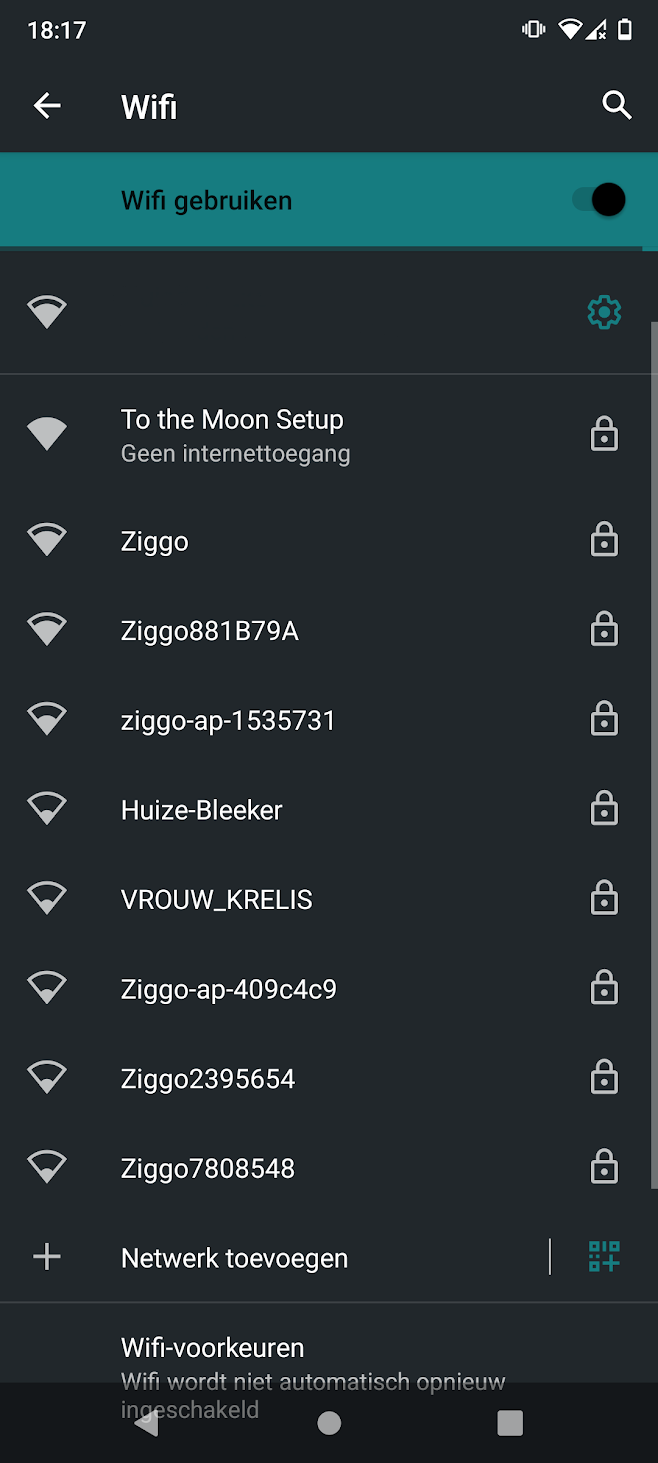
\includegraphics[width=0.7\textwidth]{step_2}
            \caption{Connect to the Wifi access point, ``To the moon setup''}
            \label{fig:step_2}
        \end{minipage}\hfill
        \begin{minipage}{0.45\textwidth}
            \centering
            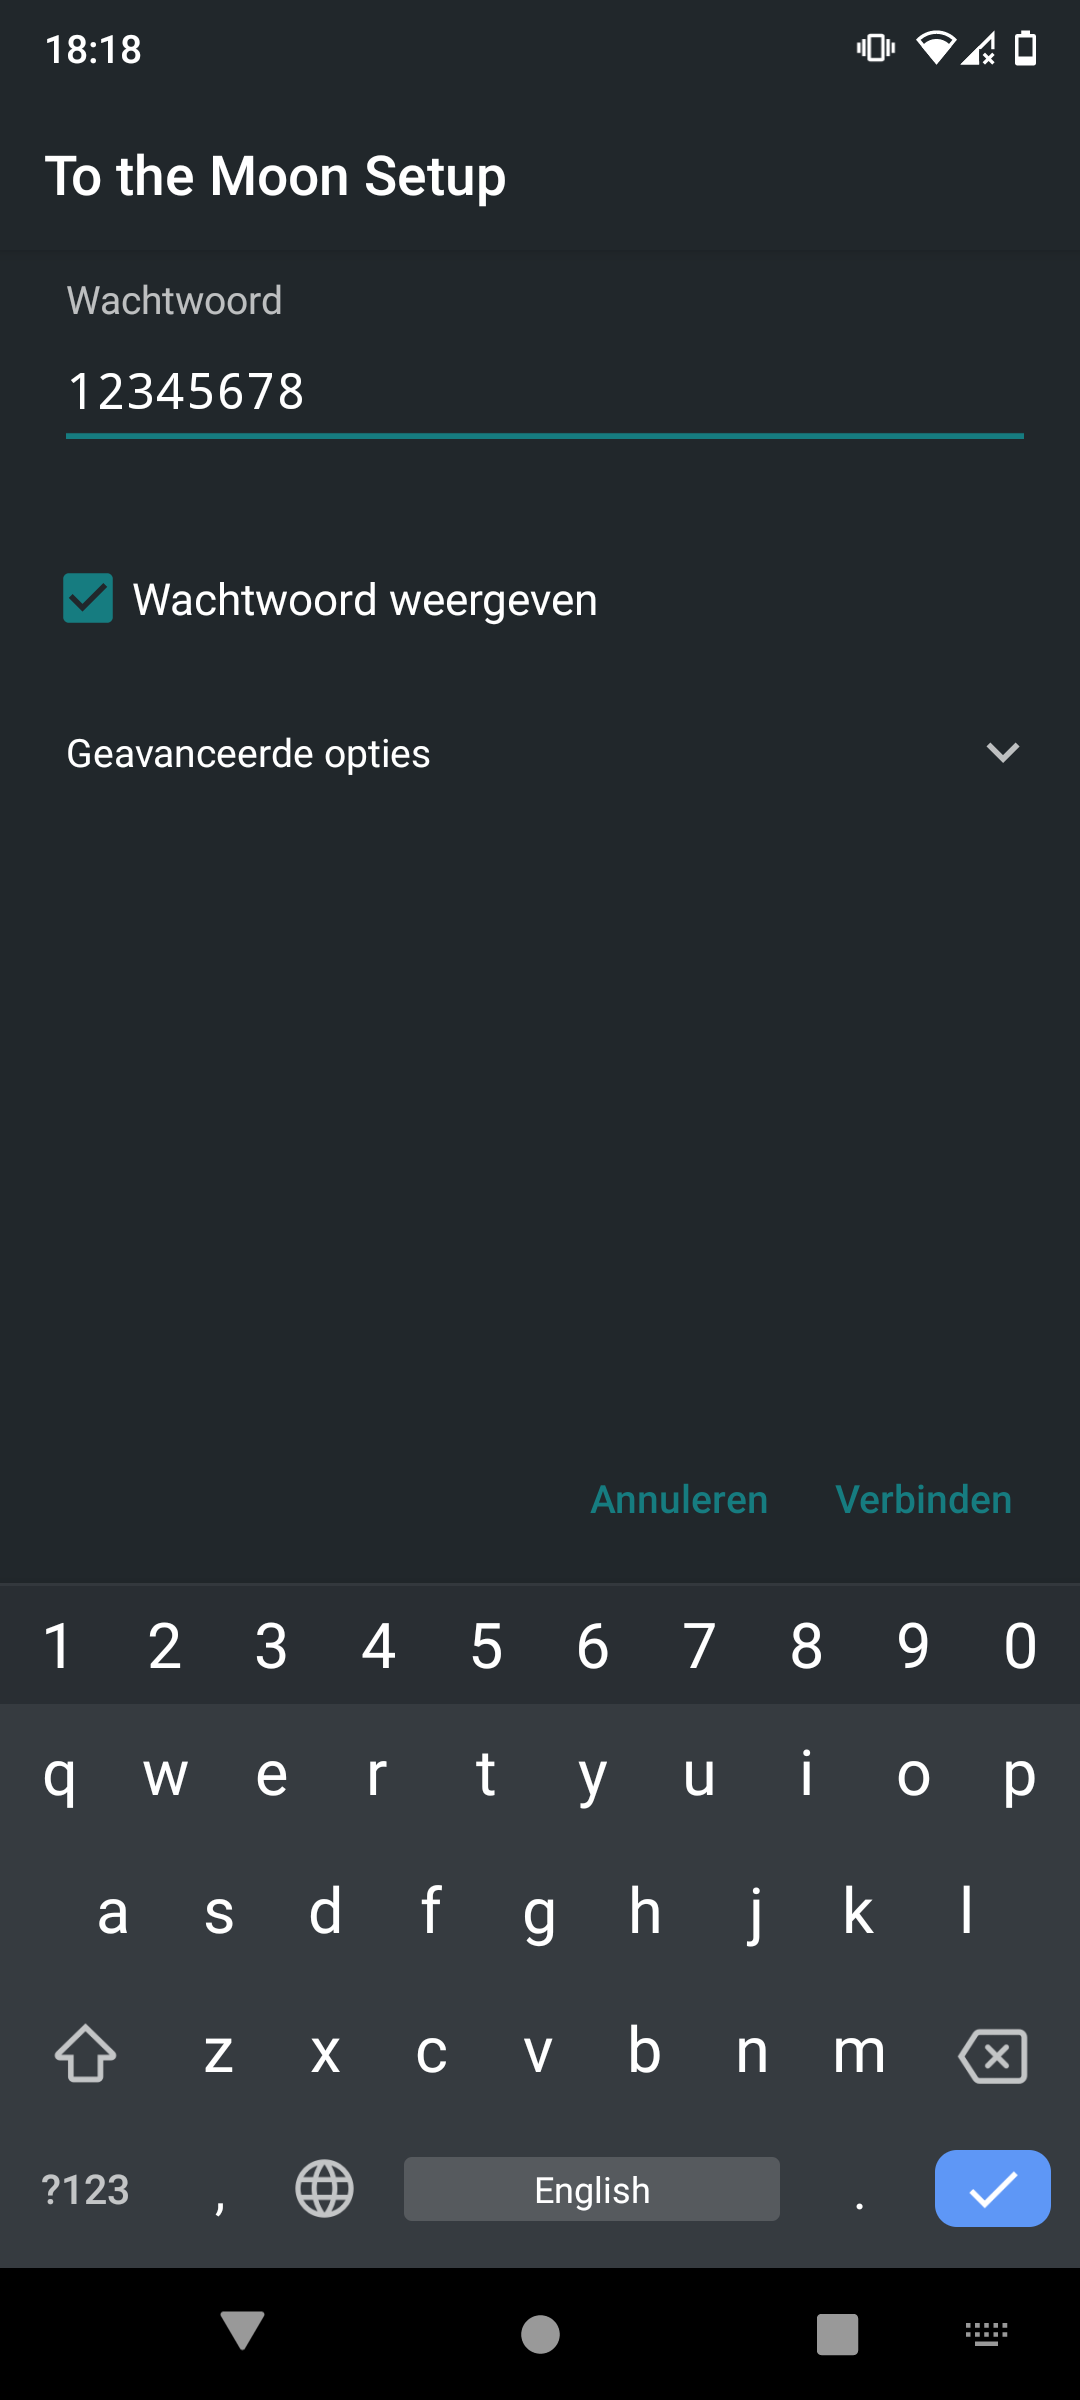
\includegraphics[width=0.7\textwidth]{step_3}
            \caption{Fill in the password ``12345678'', and connect to the access point}
            \label{fig:step_3}
        \end{minipage}
    \end{figure}
    \newpage
    \paragraph{4} When connected, open your browser and navigate to \verb!192.168.1.1! in the search bar~(\textcolor{blue}{\cref{fig:step_5}}).
    \paragraph{5} You will get a website, here you can enter the information needed to connected to your home Wifi network.
    When you have filled in the network information you press the "submit" button~(\textcolor{blue}{\ref{fig:step_6}}).
    \begin{figure}[H]
        \centering
        \begin{minipage}{0.45\textwidth}
            \centering
            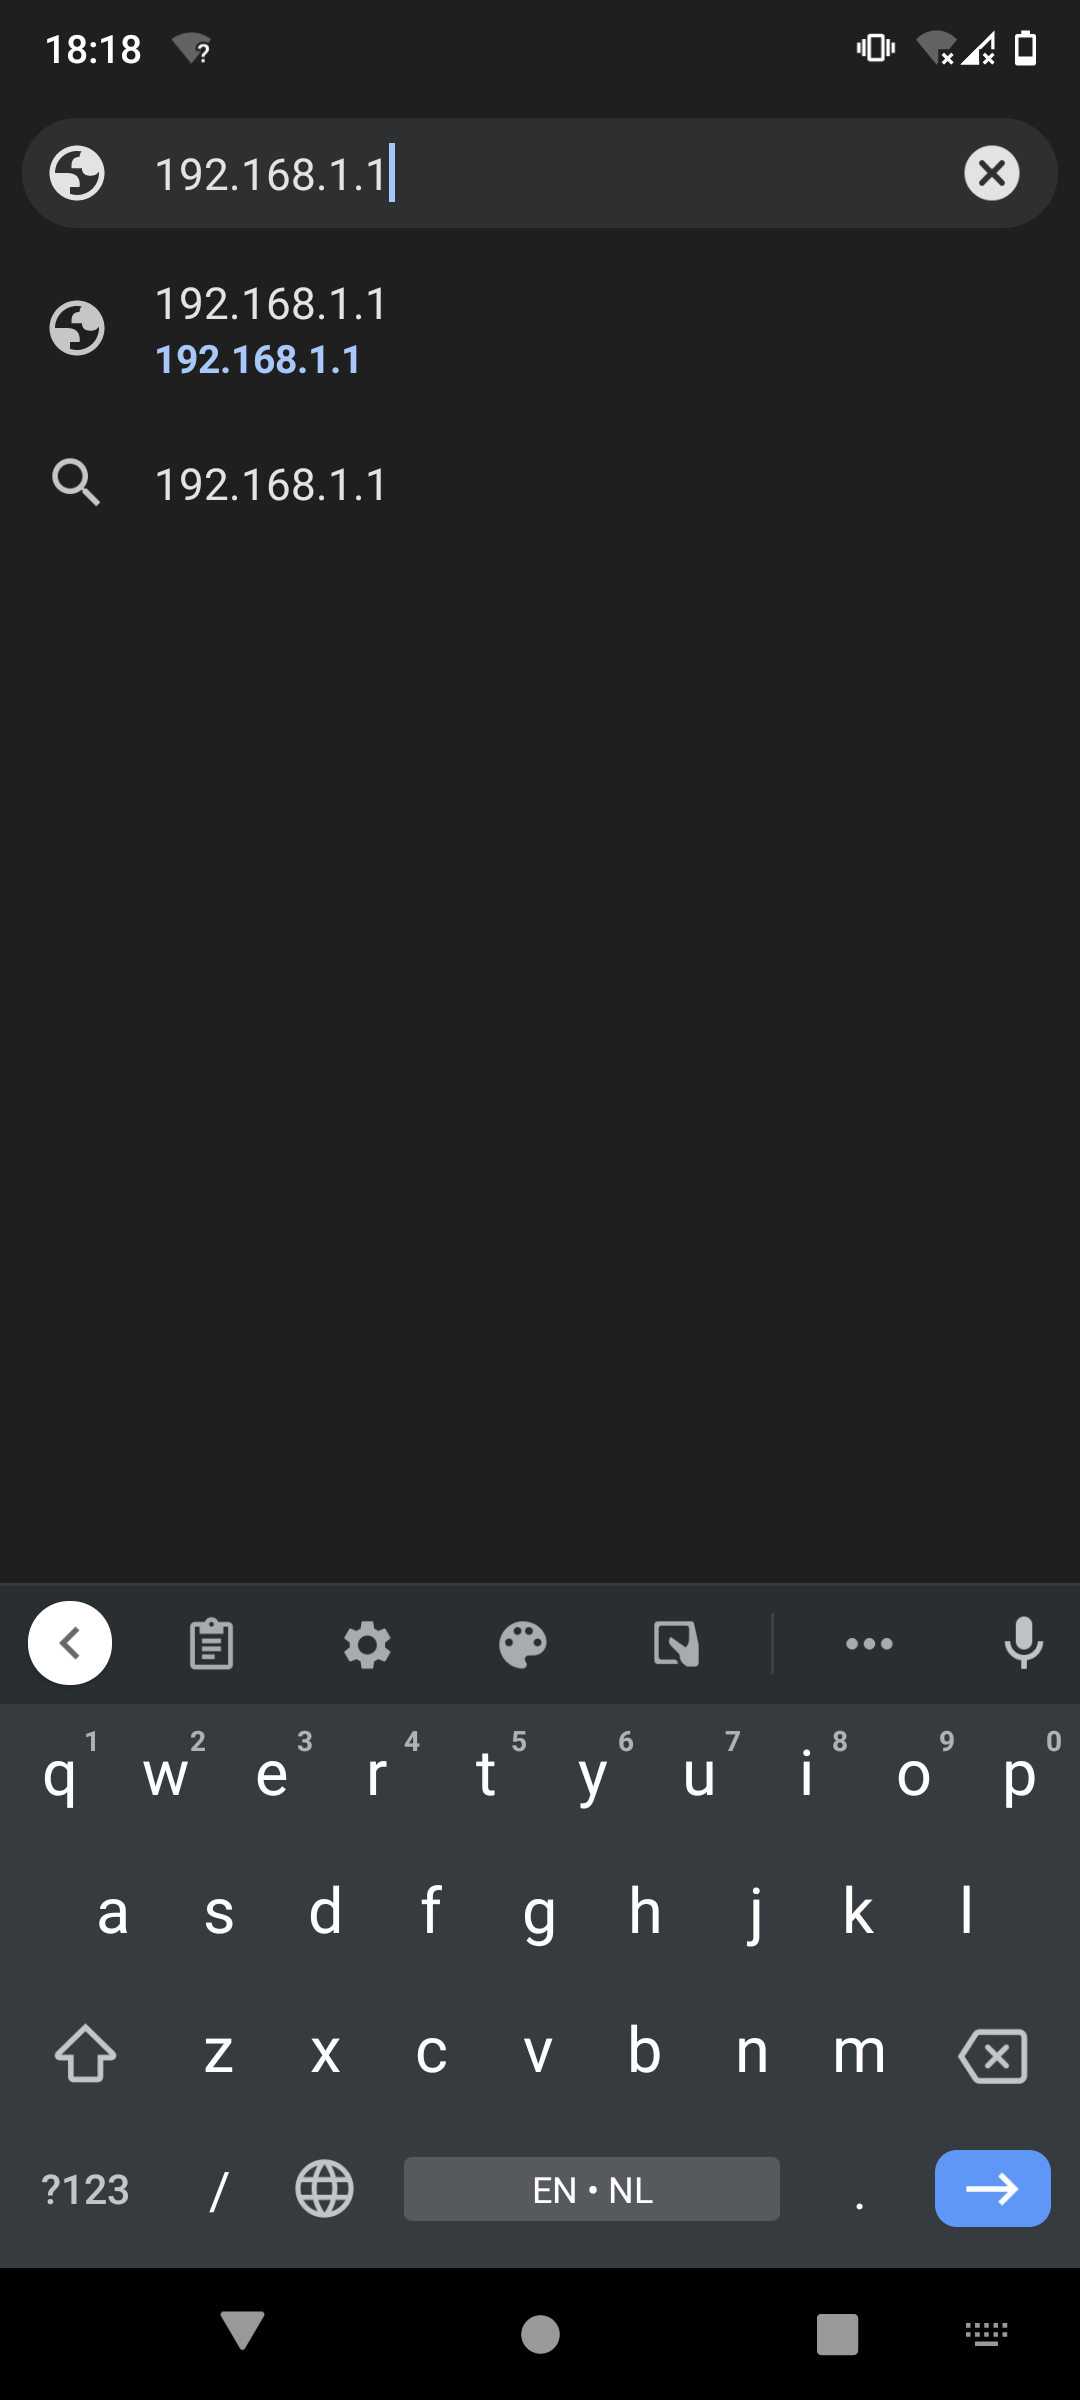
\includegraphics[width=0.7\textwidth]{step_5}
            \caption{navigate to "192.168.1.1" using your browser}
            \label{fig:step_5}
        \end{minipage}\hfill
        \begin{minipage}{0.45\textwidth}
            \centering
            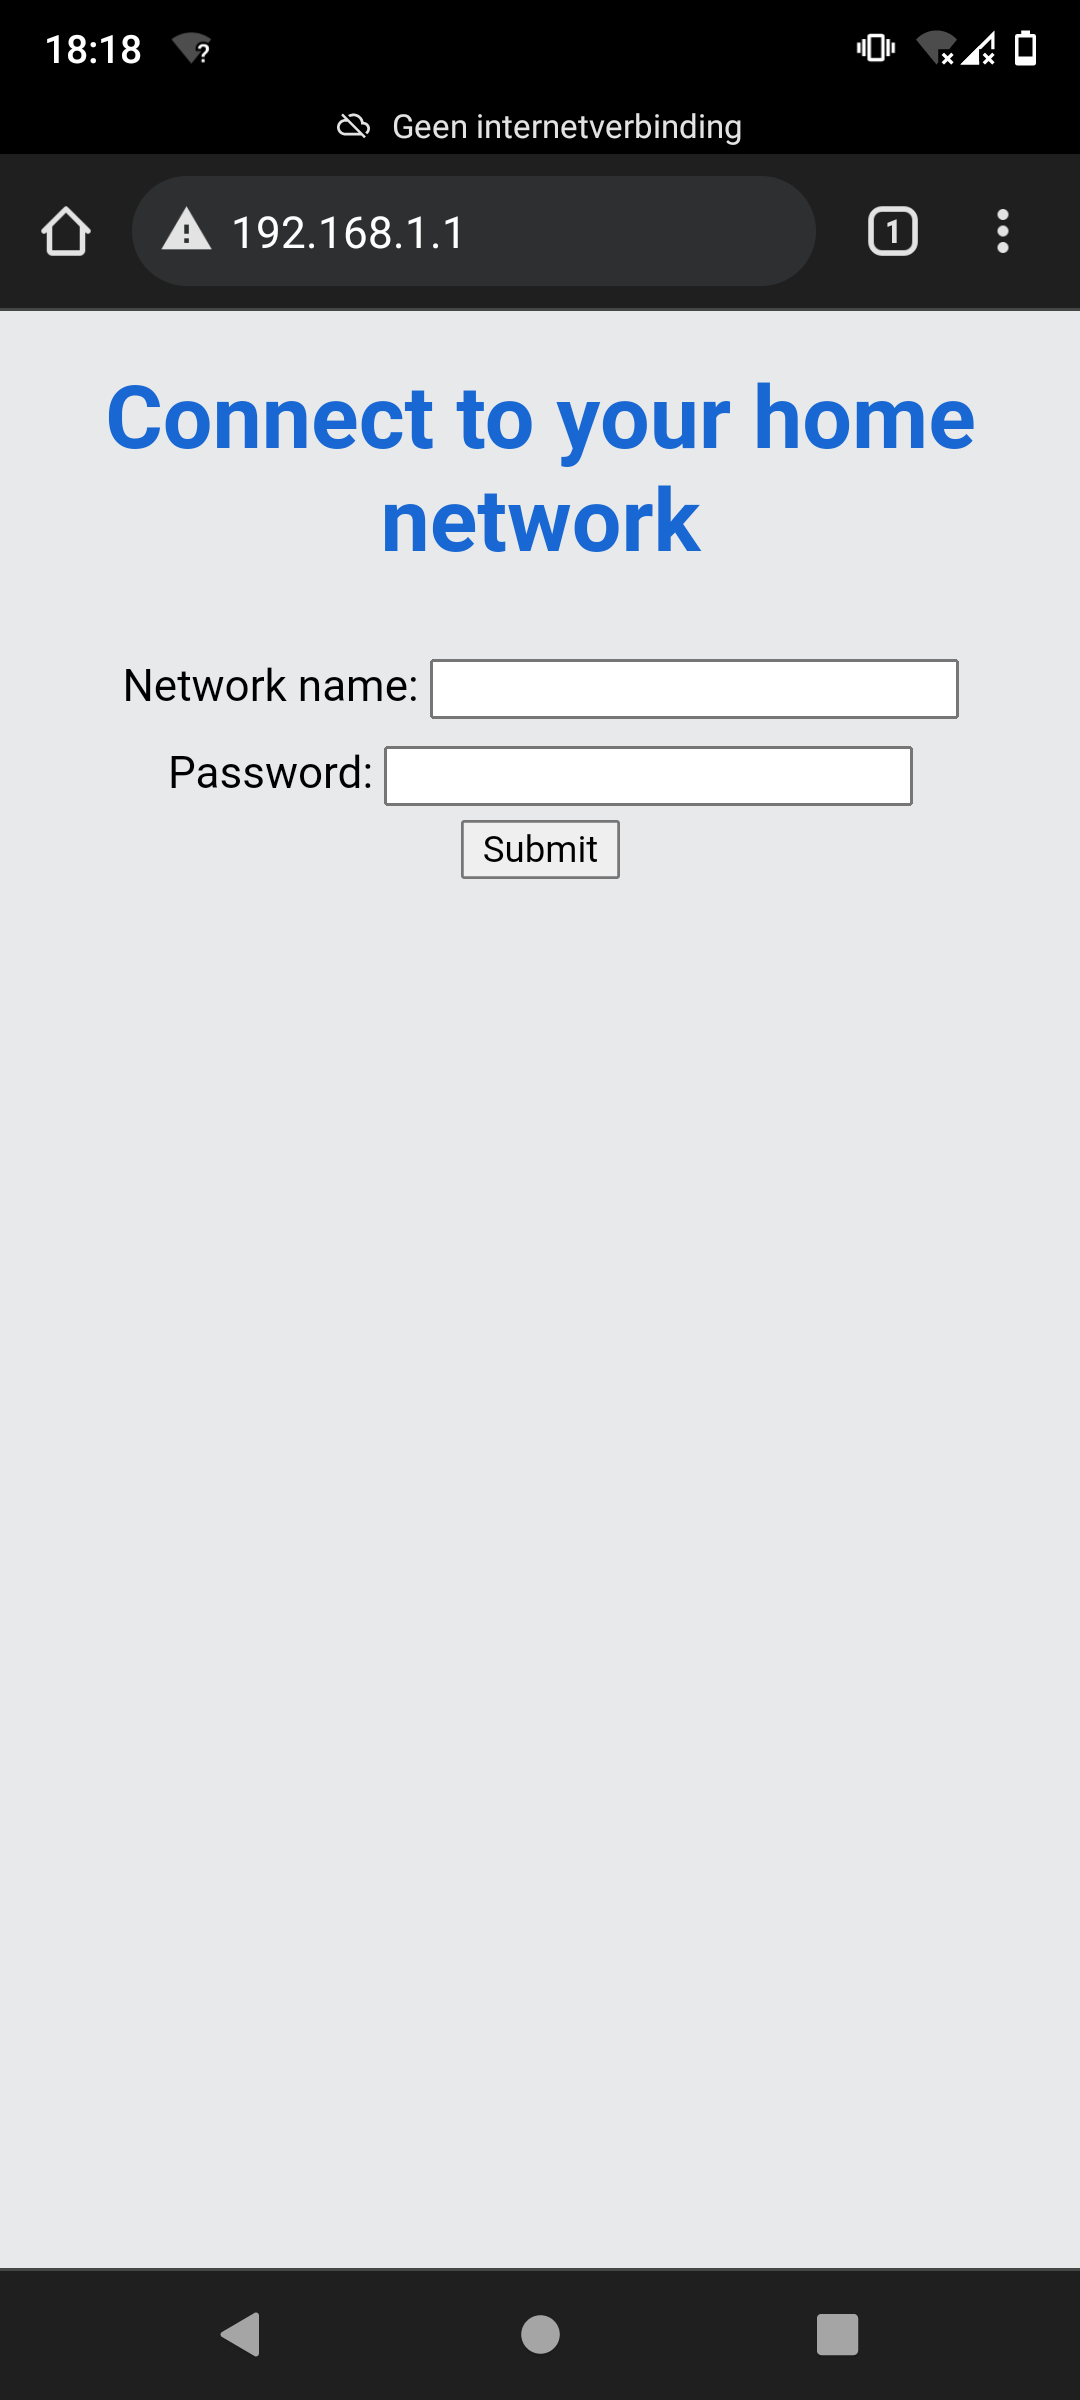
\includegraphics[width=0.7\textwidth]{step_6}
            \caption{Enter the information needed to connected to your home Wifi}
            \label{fig:step_6}
        \end{minipage}
    \end{figure}

    \paragraph{6} Restart the device, if the first setup page is shown~(\textcolor{blue}{\cref{fig:firt_setup}}) still shows up, it is possible there was a fault in the network name and or password.
    Please reconnect to the access point and resubmit the information.

    \newpage
    \section{Adding or removing a coin to the Crypt-o-meter}\label{sec:adding-or-removing-a-coin-to-the-Crypt-o-meter}
    When the devices is able to connect to your home network, it is time to add some coins you want to track with your Crypt-o-meter.
    After you have powered off and on the device the Crypt-o-meter will show a IP adress on the screen, the IP adress is only there for a few seconds on start up.
    This IP adress is the adress where you can find the website of the Crypt-o-meter.
    To visit the website, follow the same steps as shown in~\textcolor{blue}{\cref{fig:step_5}}.

    You will see the following:
    \begin{figure}[H]
        \centering
        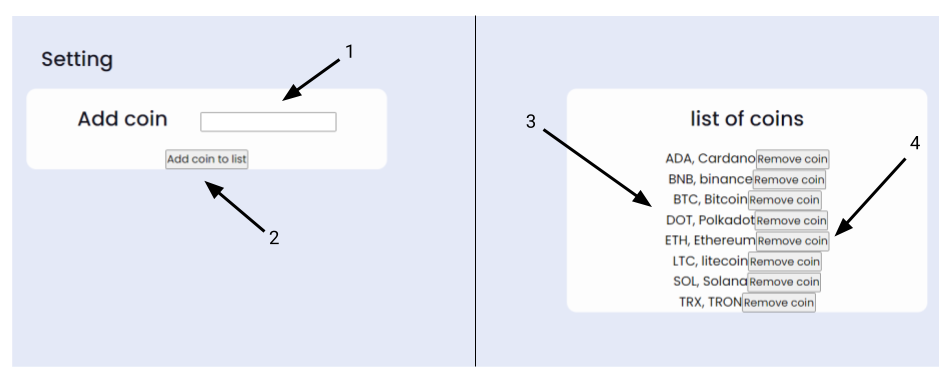
\includegraphics[width=\textwidth]{webserver}
        \caption{}
        \label{fig:webserver}
    \end{figure}

    The website consist of two parts, on the left side, you can add a coin to keep track off.
    On the right, you see a overview of the coins that have already been added to the Crypt-o-meter~\textcolor{blue}{(3 in \cref{fig:webserver})}.
    The Crypt-o-meter can keep track up to \textbf{8 crypto coins}.

    \subsection{Add coin}\label{subsec:add-coin}
    To add a coin, fill the ID of the coin in the iput field~\textcolor{blue}{(1 in \cref{fig:webserver})}.
    And then press ``Add coin to list''~\textcolor{blue}{(2 in \cref{fig:webserver})}.
    When a valid ID was entered and the website approved the the ID, it will add it to the Crypt-o-meter and starts tracking it.
    The website is automatically reloaded, and the newly added coin will show up in the list on the right side of the website~\textcolor{blue}{(3 in \cref{fig:webserver})}.

    \subsection{Remove coin}\label{subsec:remove-coin}
    To remove a coin, simply press the ``Remove coin'' beside the information of the coin~\textcolor{blue}{(4 in \cref{fig:webserver})}.
    The website is automatically reloaded, and the coin will be removed from the Crypt-o-meter.

    \newpage

    \section{User Interface of the Crypt-o-meter}\label{sec:user-interface-crypt-o-meter}
    When the Crypt-o-meter is successfully setup and coins are added, after a restart the Crypt-o-meter will plot the user interface (see~\textcolor{blue}{\cref{fig:main_UI}}).

    \begin{figure}[H]
        \centering
        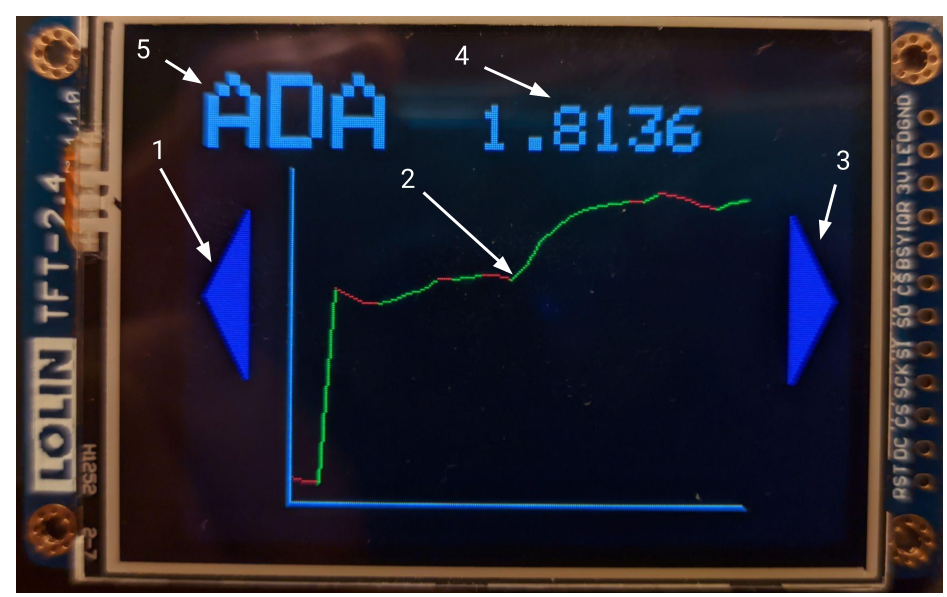
\includegraphics[width=\textwidth]{screen_1}
        \caption{Main user interface}
        \label{fig:main_UI}
    \end{figure}

    \begin{enumerate}
        \item Step up in the list of the coins being tracked
        \item The graph that represents the raise and fall of the value of a coin
        \item Step down in the list of the coins being tracked
        \item Most resent price of a coin
        \item The ID of the coin, in example (ADA, Cardano)
    \end{enumerate}

    When you press on the graph you will be presented with a pop up dialog, in that you find the maximum price and the minimum price of the coin.
    And the differents between the first and last point in the graph is presented in a percentual growth, (see~\textcolor{blue}{\cref{fig:pop_ui}}).

    \begin{figure}[H]
        \centering
        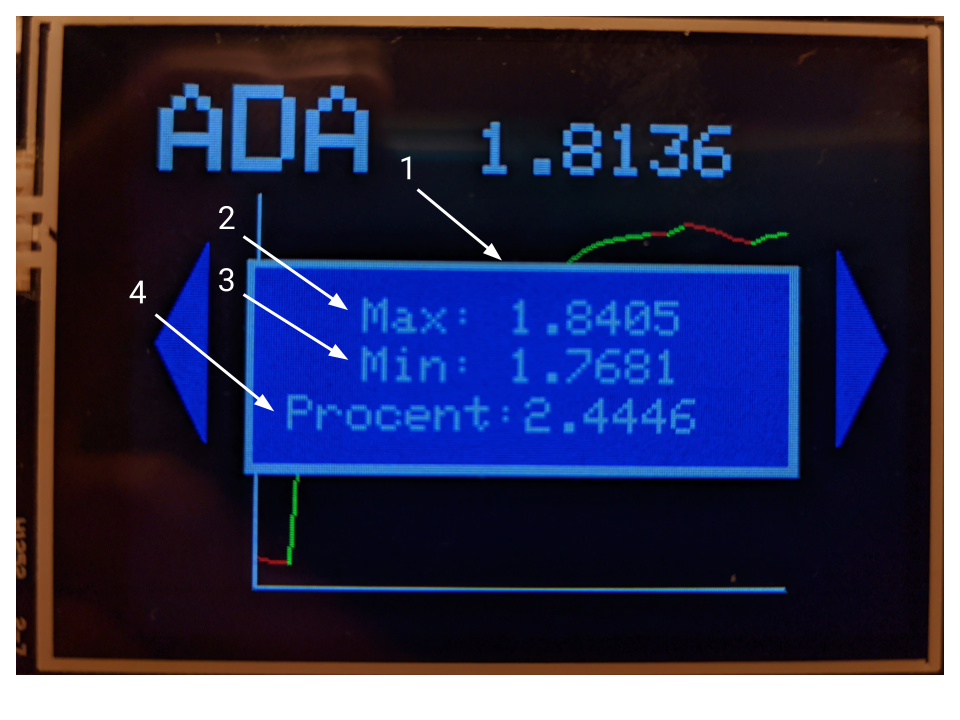
\includegraphics[width=\textwidth]{screen_2}
        \caption{Main user interface}
        \label{fig:pop_ui}
    \end{figure}

    \begin{enumerate}
        \item Pop up dialog
        \item Max price of the coin in the graph
        \item Min price of the coin in the graph
        \item Percentual growth of the coin
    \end{enumerate}

    \newpage

    \section{Resetting the Crypt-o-meter}\label{sec:resetting-the-crypt-o-meter}
    When you want to reset the Crypt-o-meter, because you want to connect to a different Wifi network.
    Press the button on the back of the Crypt-o-meter will powering it on.
    This button is located near the B mini usb port.
    This will remove any data saved on the Crypt-o-meter, and it will startup just like new.


\end{document}